\subsubsection{Storage Management}
To make database engines easy to use, some abstractions have to happen.
\begin{figure}[h!]
    \begin{center}
        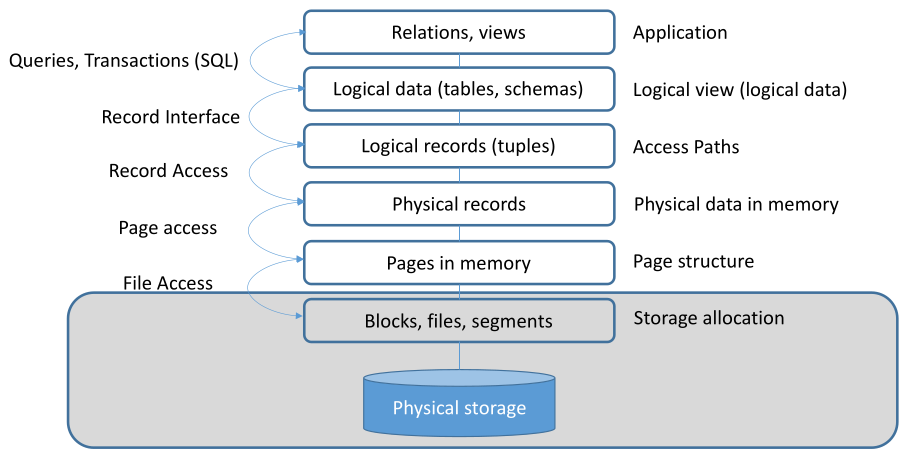
\includegraphics[width=0.7\textwidth]{assets/db-system-memory.png}
    \end{center}
    \caption{Overview of a typical abstraction for a database system
        (Figure from lecture slides 09, slide 3)}
\end{figure}

In the design of database engines it is commonly assumed that the data is stored on spinning disks, i.e. HDDs, with a high latency for seeks (random accesses)
and that most of the DB is not in memory.

Very modern database systems may assume that a higher percentage of the DB is stored in memory due to the higher quantity of memory available,
as well as lower access latencies due to the more readily available SSDs and high-speed NASes.

Some database systems operate similarly to operating systems in certain aspects, in that they manage their own processes and all of the memory
to get the absolute maximum performance out of the systems.
